%%%%%%%%%%%%%%%%%%%%%%%%%%%%%%%%%%%%%%%%%
% Beamer Presentation
% LaTeX Template
% Version 1.0 (10/11/12)
%
% This template has been downloaded from:
% http://www.LaTeXTemplates.com
%
% License:
% CC BY-NC-SA 3.0 (http://creativecommons.org/licenses/by-nc-sa/3.0/)
%
%%%%%%%%%%%%%%%%%%%%%%%%%%%%%%%%%%%%%%%%%

%----------------------------------------------------------------------------------------
%	PACKAGES AND THEMES
%----------------------------------------------------------------------------------------

\documentclass{beamer}

\mode<presentation> {

% The Beamer class comes with a number of default slide themes
% which change the colors and layouts of slides. Below this is a list
% of all the themes, uncomment each in turn to see what they look like.

%\usetheme{default}
%\usetheme{AnnArbor}
%\usetheme{Antibes}
%\usetheme{Bergen}
%\usetheme{Berkeley}
%\usetheme{Berlin}
%\usetheme{Boadilla}
\usetheme{CambridgeUS}
%\usetheme{Copenhagen}
%\usetheme{Darmstadt}
%\usetheme{Dresden}
%\usetheme{Frankfurt}
%\usetheme{Goettingen}
%\usetheme{Hannover}
%\usetheme{Ilmenau}
%\usetheme{JuanLesPins}
%\usetheme{Luebeck}
%\usetheme{Madrid}
%\usetheme{Malmoe}
%\usetheme{Marburg}
%\usetheme{Montpellier}
%\usetheme{PaloAlto}
%\usetheme{Pittsburgh}
%\usetheme{Rochester}
%\usetheme{Singapore}
%\usetheme{Szeged}
%\usetheme{Warsaw}

% As well as themes, the Beamer class has a number of color themes
% for any slide theme. Uncomment each of these in turn to see how it
% changes the colors of your current slide theme.

%\usecolortheme{albatross}
%\usecolortheme{beaver}
%\usecolortheme{beetle}
%\usecolortheme{crane}
\usecolortheme{dolphin}
%\usecolortheme{dove}
%\usecolortheme{fly}
%\usecolortheme{lily}
%\usecolortheme{orchid}
%\usecolortheme{rose}
%\usecolortheme{seagull}
%\usecolortheme{seahorse}
%\usecolortheme{whale}
%\usecolortheme{wolverine}

%\setbeamertemplate{footline} % To remove the footer line in all slides uncomment this line
%\setbeamertemplate{footline}[page number] % To replace the footer line in all slides with a simple slide count uncomment this line

%\setbeamertemplate{navigation symbols}{} % To remove the navigation symbols from the bottom of all slides uncomment this line
}

\usepackage{graphicx} % Allows including images
\usepackage{booktabs} % Allows the use of \toprule, \midrule and \bottomrule in tables

%----------------------------------------------------------------------------------------
%	TITLE PAGE
%----------------------------------------------------------------------------------------

\title[VE216]{VE216 Recitation Class 1} % The short title appears at the bottom of every slide, the full title is only on the title page

\author{ZHU Yilun} % Your name
\institute[SJTU] % Your institution as it will appear on the bottom of every slide, may be shorthand to save space
{
UM-SJTU Joint Institute \\ % Your institution for the title page
\medskip
\textit{VE216 SU20 Teaching Group} % Your email address
}
\date{2020 Summer} % Date, can be changed to a custom date e.g.:\today

\begin{document}

\begin{frame}
\titlepage % Print the title page as the first slide
\end{frame}

\begin{frame}
\frametitle{Overview} % Table of contents slide, comment this block out to remove it
\tableofcontents % Throughout your presentation, if you choose to use \section{} and \subsection{} commands, these will automatically be printed on this slide as an overview of your presentation
\end{frame}

%----------------------------------------------------------------------------------------
%	PRESENTATION SLIDES
%----------------------------------------------------------------------------------------

%------------------------------------------------
\section{Introduction} % Sections can be created in order to organize your presentation into discrete blocks, all sections and subsections are automatically printed in the table of contents as an overview of the talk
%------------------------------------------------

\subsection{RC Arrangement} % A subsection can be created just before a set of slides with a common theme to further break down your presentation into chunks

\begin{frame}
\frametitle{RC Arrangement}
\begin{table}
\begin{tabular}{ l l}
\toprule
\textbf{Time} & \textbf{Join Through}\\
\midrule
Monday 16:00 - 17:30 & Zoom ID: 537 259 5052 \\
\bottomrule
\end{tabular}
\end{table}

For zoom RC:
\begin{itemize}
    \item you may need to join twice, due to 40-min limit
    \item I will join only 5 min before class starts, due to 40-min limit
    \item If you have questions, I prefer: \\
    Raise hand, then speak $>$ public message $>$ private message 
\end{itemize}

For TA's job:
\begin{itemize}
    \item ZHU Yilun - RC 
    \item CHEN Ling, LI Zhipeng, YUAN Shuai - all the other staff, including Homework, Quiz, Lab, ...
    \item Please contact by email, rather than via Wechat
\end{itemize}

\end{frame}


\subsection{General Advice}
\begin{frame}
\frametitle{General Advice}
\begin{itemize}
\item To me, this course seems like an (Applied) Math course, therefore:
    \begin{itemize}
        \item Don't get lost in Math, think about physical meaning 
        \item Live with ambiguousness, don't treat it as a ``Theoretical'' Math course
    \end{itemize}
\item The course ``Signals and Systems'' on MIT Open Courseware by Prof. Alan V. Oppenheim's is highly recommended
\begin{itemize}
    \item Personally, recommend Video Lecture $>$ Textbook 
\end{itemize}

\item This course is inspiring because it provides a different view
\begin{itemize}
    \item When I first study this course, the application to \emph{Communication Systems} is really fascinating to me.
    \item After working as TA and reviewed all the contents again, I realized that this course is full of brilliant ideas.
    \item I hope, at least, tell you the points that attracted me most
\end{itemize}

\item Ever think of why this course is titled ``Signals and Systems''?

\end{itemize}
\end{frame}

%------------------------------------------------




%------------------------------------------------
\section{Chapter 1: Signals and Systems}
%------------------------------------------------

%------------------------------------------------
\subsection{Signal Characteristics}
%------------------------------------------------
\begin{frame}
\frametitle{Even and Odd}
\begin{theorem}[Even and odd components]
\begin{displaymath}
x(t) = x_e(t) + x_o(t)
\end{displaymath}
\begin{displaymath}
x_e(t) = \frac{1}{2}[x(t)+x(-t)], x_o(t) = \frac{1}{2}[x(t)-x(-t)]
\end{displaymath}
\end{theorem}
\end{frame}
%------------------------------------------------

\begin{frame}
\frametitle{Energy and Power}
\begin{itemize}
\item Do not cram. Remember with the help of graph. (Eg.: power consumed by a resistor)    
\item Average value: \[A = \lim_{T \rightarrow \infty} \frac{1}{2T} \int_{-T}^{T} x(t)dt\]
\item Energy (remember the square): \[E = \int_{-\infty}^{\infty} |x(t)|^2 dt \]
\item Average power: \[P = \lim_{T \rightarrow \infty} \frac{1}{2T} \int_{-T}^{T} |x(t)|^2dt\]
\item Energy Signal, Power Signal 

\end{itemize}
\end{frame}
%------------------------------------------------
\subsection{Singularity Functions}

\begin{frame}
\frametitle{Singularity Functions}
\begin{itemize}
\item Unit Step Function: $u(t)$

\begin{itemize}
    \item $ \delta(t) = \frac{d}{dt} u(t) $
\end{itemize}

\item Rectangle Function: 

\begin{itemize}
    \item $rect(t)$
    \item $rect(t) = rect(-t)$
    \item $rect(\frac{t-t_0}{T})$ is centered at $t_0$ and with width $T$
\end{itemize}


\item Skill: Using these functions to represent piecewise functions --- Q4,9
\end{itemize}
\end{frame}

\begin{frame}
    \frametitle{Exercise: Q4(a)}
    \begin{figure}
        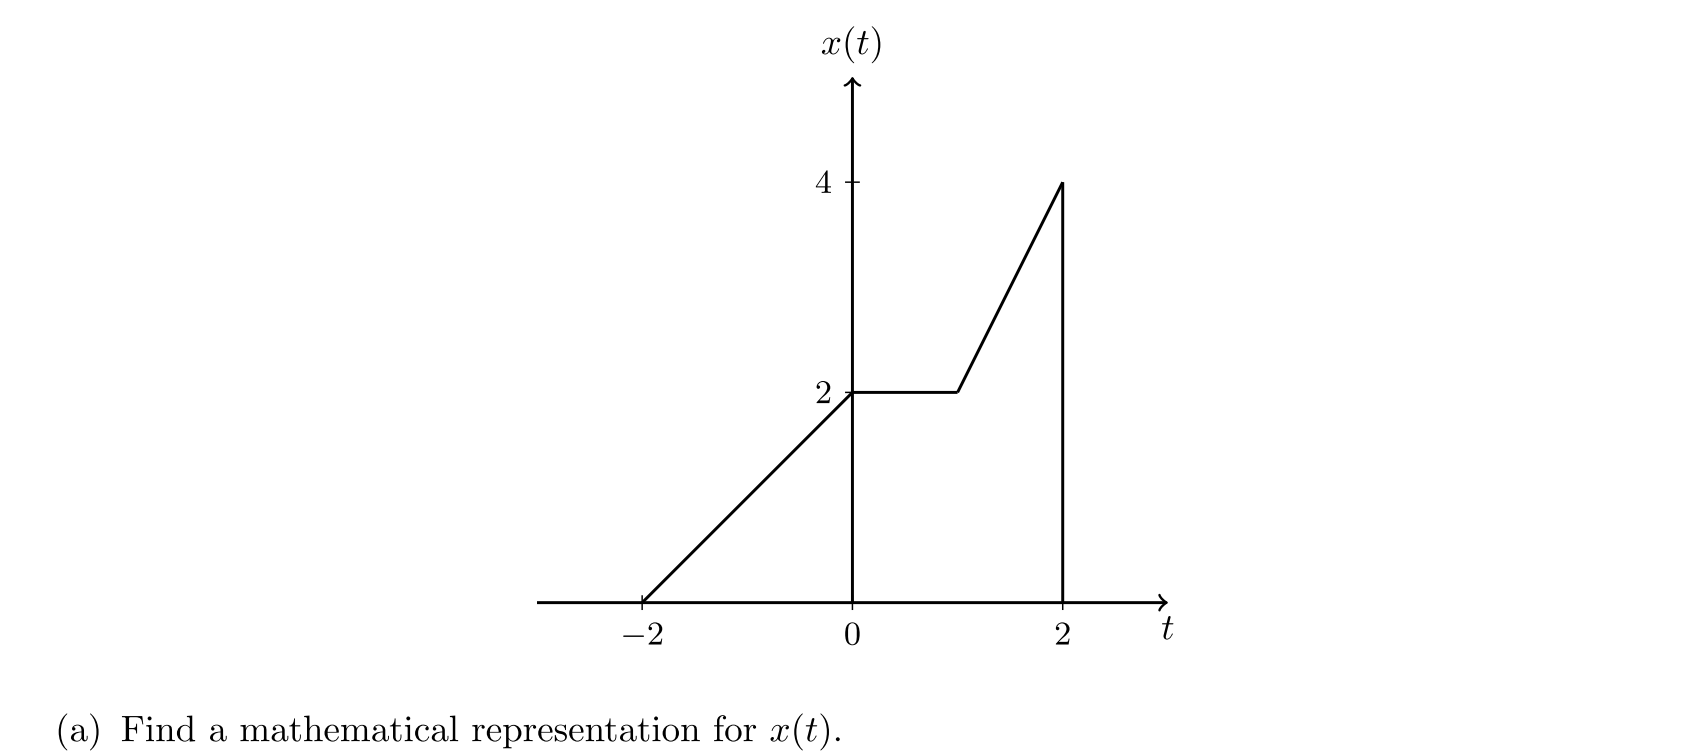
\includegraphics[width=1\linewidth]{hw1_q4}
    \end{figure}

    \bigskip
    \bigskip
    \bigskip
    \bigskip
\end{frame}


\begin{frame}
    \frametitle{Exercise: Q9}
    \begin{figure}
        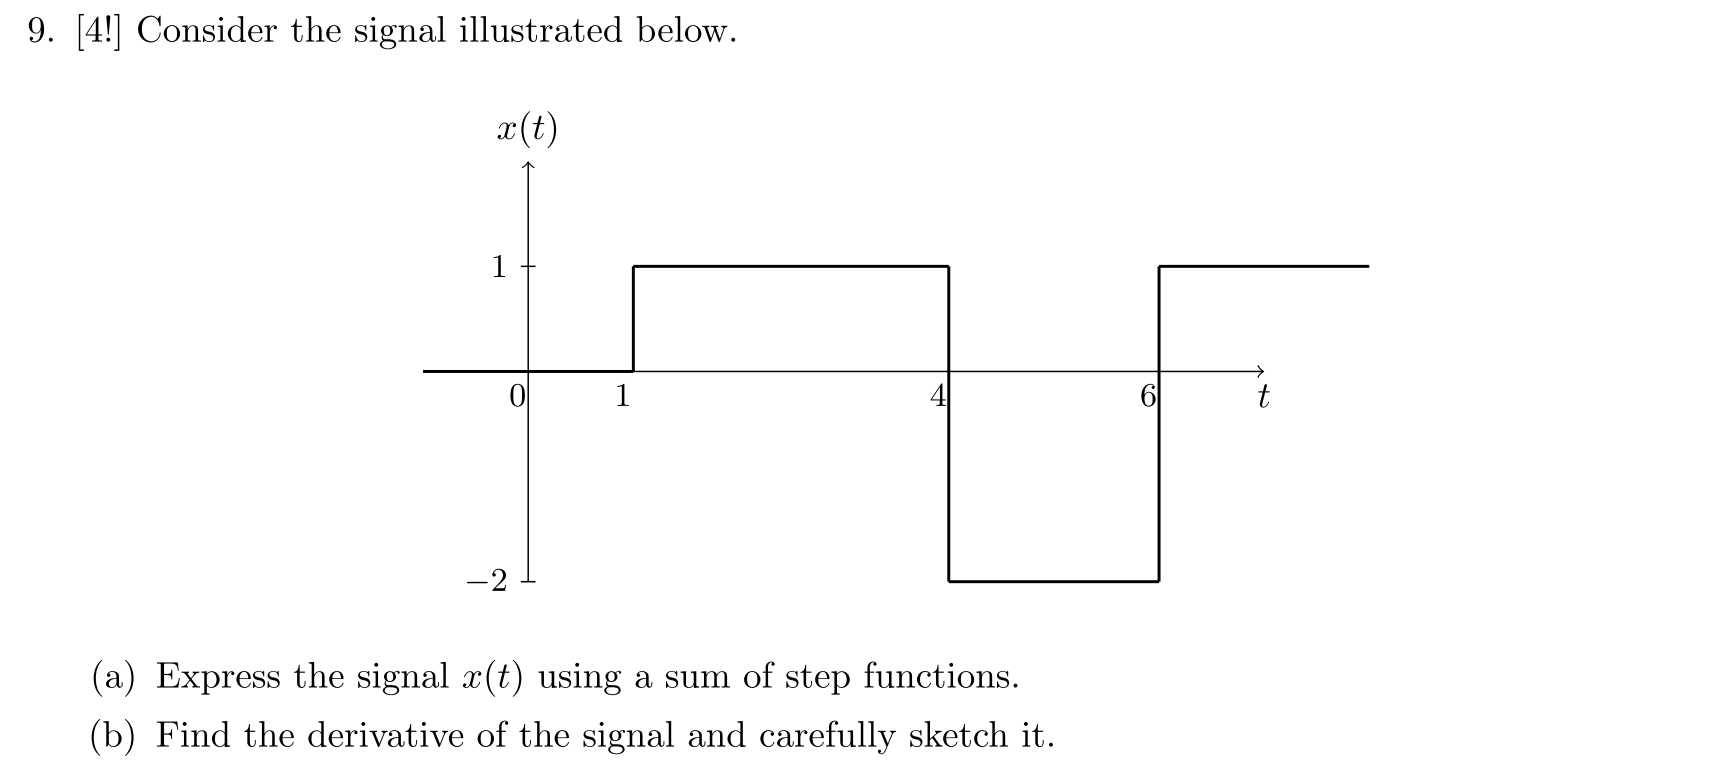
\includegraphics[width=0.9\linewidth]{hw1_q9}
    \end{figure}

    \bigskip
    \bigskip
    \bigskip
    \bigskip
    \bigskip
    \bigskip
    \bigskip
    \bigskip
\end{frame}
%-------------------------------------------------
\begin{frame}
\frametitle{Singularity Functions}
\begin{itemize}

\item Unit Impulse Function: $\delta(t)$ 
\begin{itemize}
    \item sampling property --- function \[ x(t)\delta(t - t_0) = x(t_0)\delta(t-t_0) \] 
    \item sifting property --- number \[ \int_{-\infty}^{\infty} x(t)\delta(t - t_0) dt = x(t_0)\] 
    \item scaling property (prove : using area) \[ \delta(at) = \frac{1}{|a|} \delta(t)\]     
\end{itemize}


\bigskip
    \bigskip
    \bigskip

\end{itemize}
\end{frame}

\begin{frame}
    \frametitle{Exercise}
    \begin{figure}
        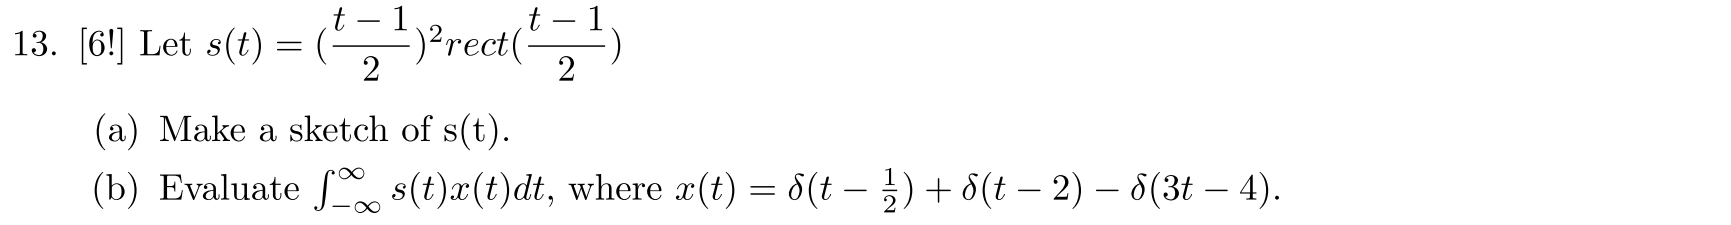
\includegraphics[width=1\linewidth]{hw1_q13}
    \end{figure}

    \bigskip
    \bigskip
    \bigskip
    \bigskip
    \bigskip
    \bigskip
    \bigskip
    \bigskip
\end{frame}
%-------------------------------------------------

\subsection{Transformation of Signals}

\begin{frame}
\frametitle{Transformation of Signals}
\begin{theorem}[Time transformation]
$1) \quad x(\frac{t-t_0}{w}) \qquad 2) \quad x(at-b)$
\end{theorem}
For Graph: \\
1) First scale according to $w$, then shift according to $t_0$ \\
2) First time-delay by $b$, then time-scale by $a$ 
\newline \\
Wait... The word ``Transformation'' sounds familiar? \\
Yes. Transformation of signals is performed by systems! 
\newline 
\newline
Think about the physical meaning: 
There are two systems, one can shift the time, another can scale the time. Different sequence of connection requires different specification of ($w, t_0, a, b$) to reach the same effect. 
%\newline \\
%Question: are they casual, time-invariant, linear?
\end{frame}

\begin{frame}
    \frametitle{Transformation of Signals}
    \begin{theorem}[Amplitude transformation]
    1) Reversal $y(t) = -x(t) $ \\
    2) Scaling $y(t) = ax(t)$ \\
    3) Shifting $y(t) = x(t) + b $\\
    \end{theorem}  
\end{frame}
    
\begin{frame}
    \frametitle{General Transformation}
    \begin{itemize}
    \item ``Time'' transformation: $ y(t) = x(g(t)) $ \\
    \item ``Amplitude'' transformation: $ y(t) = h(x(t)) $ \\
    \end{itemize}
Consider:
    \begin{itemize}
    \item 1) $y(t) = x(t) $
    \item  2) $y(t) = x(\sin(t))$   
    \item  3) $y(t) = \cos(x(t))$ 
    \item 4) $y(t)=\int_{-\infty}^{t/2}x(\tau)d\tau$               
    \end{itemize}
Question: \\
    \quad Think about whether the system that perform such transformation are: \\
    \quad ``linear, stable; time-invariant, causal, memoryless'' in general.  \\
We will come back to these after going through the system properties.
\end{frame}


\subsection{Preview: Systems}

\begin{frame}
    \frametitle{Preview: Systems}
\begin{itemize}
    \item Transform the input signal to the output signal
    \item Understand the system in terms of input-output relation
    \item const. system $y(t) = 0$ vs. ``non-causal'' $ y(t) = x(t+1) - x(t+1)$?
    \bigskip
    \bigskip
    \item Question from class: Is a system casual if ``x(t)'' is non-casual?
    \bigskip
    \bigskip
    \bigskip
    \item Digression: physical meaning of knowing $x(t)$, e.g.: $x(t) = \sin(t)$?
\end{itemize}

\end{frame}

%------------------------------------------------
\section{Summary}
\begin{frame}
    \frametitle{Summary}
    \begin{itemize}
        \item Singularity functions
        \item Connection between signals and systems
        \item 2nd RC will focus on system properties
        
    \end{itemize}
    
\end{frame}

%------------------------------------------------

\begin{frame}
\Huge{\centerline{The End}}
%\huge{\centerline{See you next Thursday}}
\end{frame}

%----------------------------------------------------------------------------------------

\end{document} 